\documentclass{article}
\usepackage[spanish]{babel}
\usepackage[utf8x]{inputenc}
\usepackage{amsmath}
\usepackage{graphicx}
\usepackage[colorinlistoftodos]{todonotes}
\usepackage{enumitem}
\usepackage{listings}
\usepackage{filecontents}
\usepackage{verbatim}
\usepackage{eurosym}
\usepackage{setspace}
\usepackage{natbib}
\usepackage[export]{adjustbox}
\usepackage{xcolor}
\usepackage{minted}
\usepackage{algorithm}
\usepackage[noend]{algpseudocode}
\usepackage{amssymb}
\usepackage{float}
\usepackage{subfig}
\usepackage{tocloft}
\usepackage{multicol}
\usepackage{hyperref}
\hypersetup{
    colorlinks=false,
    linkcolor=blue,
    filecolor=magenta,      
    urlcolor=cyan,
}
% \usepackage[left=2.60cm, right=2.60cm, top=3.00cm, bottom=3.00cm]{geometry}
\usepackage{titlesec}

\usetikzlibrary{positioning}

\definecolor{backcolour}{HTML}{F8F8F8}

\setminted[python]{
    framesep=2mm, 
    baselinestretch=1.2, 
    bgcolor=backcolour,
    fontsize=\footnotesize,
    linenos
}

\usepackage{sectsty}

\sectionfont{\fontsize{14}{15}\selectfont}

\newcommand{\HRule}{\rule{\linewidth}{0.5mm}}

\begin{document}

%----------------------------------------------------------------------------------------
%   TITLE PAGE
%----------------------------------------------------------------------------------------

\begin{titlepage}
\begin{center}

\textsc{\LARGE University of Granada}\\[1.5cm]


\includegraphics[width=100px]{ugrlogo.png}


\vfill
\HRule \\[0.4cm]
{\huge \bfseries Occupacy Detection}\\[0.4cm]
\textsc{\Large Machine Learning Project}\\[0.5cm]
\HRule \\[1.5cm]
 

\begin{center}
    \textsc{JUAN JOSÉ MARTÍN CARA} \textit{(54146132S)} \\
    \textsc{RAFAEL SANJUAN AGUILERA} \textit{(20080674H)} \\
\end{center}

\vfill
{\large \today}\\[4cm] % Date

\vfill
\end{center}

\end{titlepage}

\newpage
\tableofcontents





~\\
~\\
~\\
\newpage

\pagenumbering{arabic}

\section{Definición del problema a resolver y enfoque elegido (comb)}

En la actualidad el mundo del internet de las cosas ha supuesto grandes avances que están llegando a nuestras casas en forma de pequeños computadores. Un problema recurrente que tienen muchos de estos diseños es que confían en el uso de una cámaras para detectar las personas que hay en una habitación.

Nuestro objetivo consiste en discernir, de una forma no intrusiva, entre habitaciones que están ocupadas, en uso, y no ocupadas. Por lo tanto nos enfrentamos ante un problema de \textit{clasificación binaria}. Para abordar este problema se usará el la base de datos llamada \textit{'Occupancy Detection Data Set'}, gratuita y abierta al publico en el  \href{https://archive.ics.uci.edu/ml/datasets/Occupancy+Detection+/}{\color{blue}portal web de la UCI}

Esta base de datos consiste en un conjunto observaciones hechas por unos sensores y luego comprobadas gracias a fotografías realizadas cada minuto para discernir la ocupación y valores de sensores que se consideraron relevantes. De modo que un factor humano aporto la clasificación a través de fotografías y se pretende usar sensores ambientales para lograr el mismo objetivo pero reducir la intrusitivad.

% \section{Definición del problema a resolver y enfoque elegido}

% Nuestro objetivo consiste en discernir entre inmuebles que están ocupados, en uso, y los cuales no están siendo ocupados. Por lo tanto nos enfrentamos ante un problema de \textit{clasificación binaria}. Para abordar este problema se usará el la base de datos llamada \textit{"Occupancy Detection Data Set"},  gratuita y abierta al publico en el portal web de la UCI \textcolor{blue}{ref}.

% Esta base de datos consiste en observaciones sacadas de fotografías realizadas cada minuto para discernir la ocupación y valores de sensores que se consideraron relevantes.

% \section{Definición del problema a resolver y enfoque elegido (alternativa)}

% En la actualidad el mundo del internet de las cosas ha supuesto grandes avances que están llegando a nuestras casas en forma de pequeños computadores. Un problema recurrente que tienen estos diseños es que confían en el uso de una cámaras para detectar las personas que hay en una habitación.

% En nuestro problema trataremos, de una forma no intrusiva, detectar las personas que se encuentran en una oficina. Para esto se hace uso de una serie de sensores que leen características del entorno, la base de datos que contiene estos datos es  \href{https://archive.ics.uci.edu/ml/datasets/Occupancy+Detection+}{Occupancy Detection Data Set .}  Siendo esta de carácter abierto para un uso público y gratuito.

\section{Codificación de los datos de entrada para hacerlos útiles a los algoritmos.}

Cada dato de entrada consiste en los siguientes atributos:
\begin{itemize}
    \itemsep0em 
    \item Fecha y hora en forato: año-mes-dia hora:minuto:segundo 
    \item Temperatura en grados celsius.
    \item Porcentaje de humedad relativa.
    \item Luminosidad, en Lux.
    \item CO2, en ppm 
    \item Ratio de Humedad, derivado de la temperatura y humedad relativa, en kgwater-vapor/kg-air 
    \item Ocupación, 0 para no ocupado, 1 para ocupado.
\end{itemize}

De modo que tenemos unas observaciones que están ligadas a una serie temporal, cada dato tomado fue medido un minuto después del anterior.

\begin{minted}{python}
X_train = genfromtxt(filepath, delimiter=',')
y_train = X_train[:,-1]
\end{minted}

La base de datos provee un fichero de datos de entrenamiento que cargamos con el código anterior y podemos comprobar que tenemos 6414 ejemplos de clase negativa y 1729 ejemplos de clase positiva. Esto produce un cierto desbalance que habrá que tener en cuenta.

Junto a estos datos de entrenamiento tenemos dos ficheros más que en el estudio de los autores \href{https://archive.ics.uci.edu/ml/datasets/Occupancy+Detection+/}{\color{blue}ref.} se usaron para validación, elección de los hiperparámetros, (con 1693 ejemplos negativos y 972 positivos) y un conjunto de test (7703 negativos y 2049 positivos)

\newpage
\section{Valoración del interés de la variables para el problema y selección de un subconjunto (en su caso).}

~\\
{\noindent \bf \large Exploración Visual de los datos}


En esta apartado veremos de forma gráfica los datos de entrada que tenemos, esto nos asegura un mejor entendimiento del problema, además de una mayor claridad a la hora de estableces relaciones entre los distintos parámetros.


Como ya hemos comentado anteriormente, los datos con los que tratamos están compuestos en forma de línea temporal, esto significa, que podrían existir relaciones entre las muestras que han ocurrido antes y después de la actual. Para ver como se desarrolla la línea temporal de cada uno de los sensores haremos un gráfico temporal con los valores de estos.

La visualización siguiente esta inspirada por (\href{https://github.com/aqibsaeed/Occupancy-Detection}{\color{blue}aqibsaeed}):

\begin{figure}[H]
    \centering
    \makebox[\textwidth]{\makebox[1.5\textwidth]{%
    \begin{minipage}{1.45\textwidth}
        \centering
        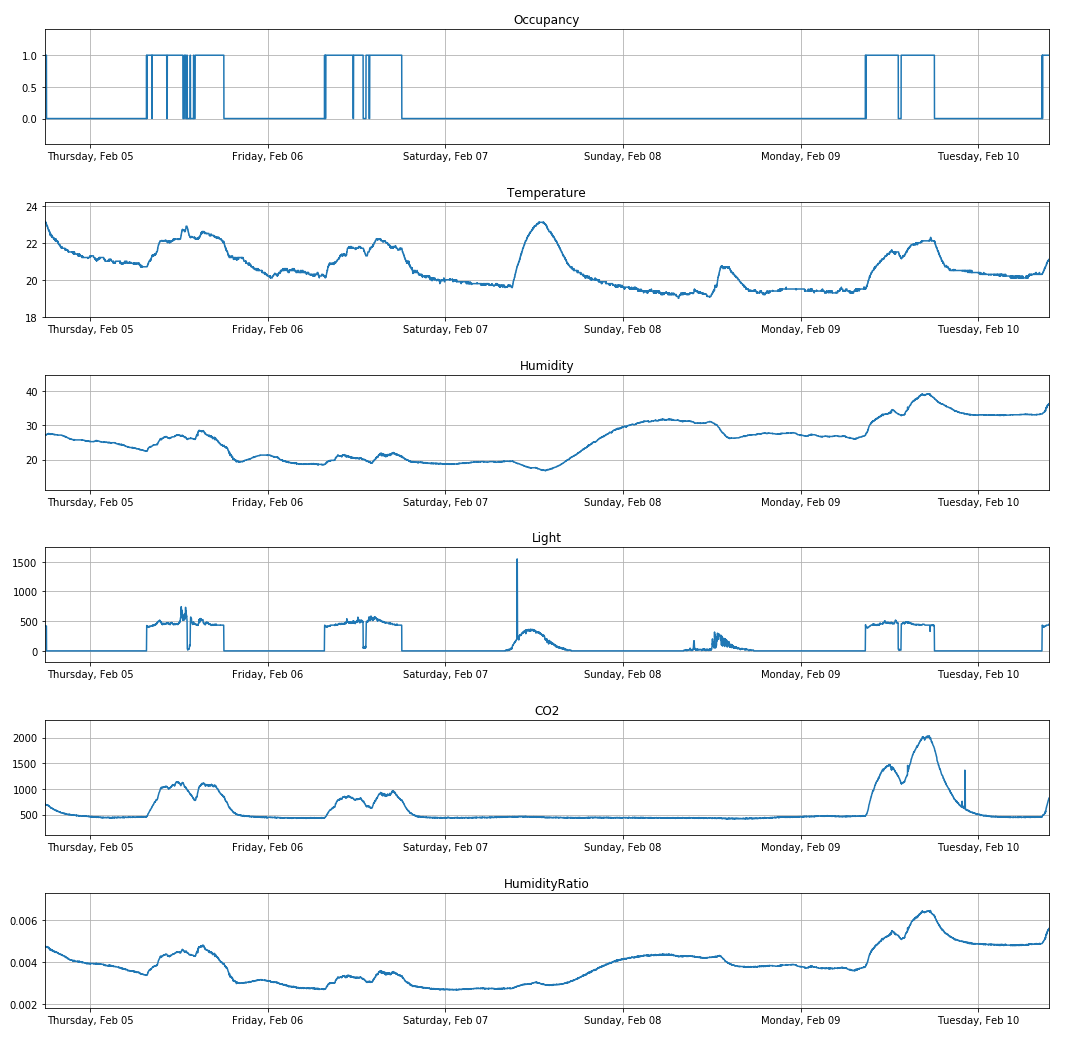
\includegraphics[width=1\textwidth]{figures/ts_plots.png}
        \caption{Visualización de las series de tiempo en cada característica}
    \end{minipage}}}
\end{figure}

Tal y como podemos ver en la figura 1, confirmamos que existen relaciones entre distintas muestras tomadas por los sensores, esto es, la localidad de cada muestra afecta al resultado de su clasificación. Como este tipo de secuencias no han sido desarrolladas en la asignatura, intentaremos realizar este proyecto sin tener en cuenta que los datos son parte de una línea temporal. Para esto, omitiremos la característica de tiempo al inicio del preprocesado y no se usará a lo largo de la práctica.

Aún así podemos comentar algunas relaciones significativas que se ven de forma clara en este tipo de gráfica. Para empezar si nos fijamos en la visualización de la característica de la temperatura junto con la ocupación, podemos ver como la temperatura, de forma general, suele elevarse al haber personas dentro de la habitación. Sin embargo, esto no significa que cada vez que suba la temperatura haya personas en la habitación.

También podemos ver como la cantidad de CO2 incrementa significativamente cuando encontramos que hay gente en la habitación. Pero para ver esto de forma más clara haremos una representación visual de los datos de forma diferente. 
\begin{figure}[H]
    \centering
    \makebox[\textwidth]{\makebox[1.35\textwidth]{%
    \begin{minipage}{1.3\textwidth}
        \centering
        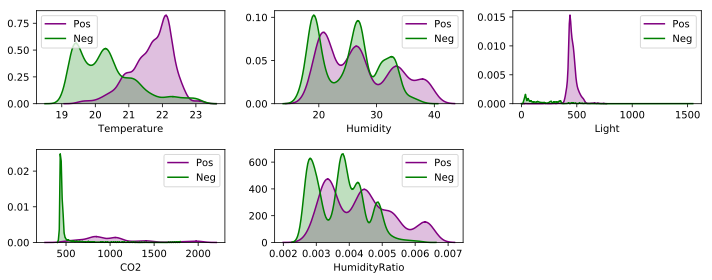
\includegraphics[width=1\textwidth]{figures/fig1}
        \caption{Visualización de cada atributo en relación con nuestro objetivo (y)}
    \end{minipage}}}
\end{figure}
Este tipo de visualización nos permite identificar en verde los valores (en el eje horizontal) que se alcanzan cuando no hay personas en la habitación y en morado los que abarca cada característica concreta al tener una habitación ocupada.

Aquí se ve de forma más sencilla como la temperatura no suele bajar de unos 20ºC cuando hay personas en la habitación y como la medida de CO2 suele ser mucho más bajo cuando no hay personas.
Estas características que tanto llaman la atención a primera vista, intuimos que serán las que más influencien de forma más notable la clasificación del modelo, sin embargo de esto hablaremos posteriormente cuando comentemos los resultados y como han sido obtenidos.

\newpage
Debido a la baja dimensionalidad de los datos, no realizaremos ninguna reducción de esta puesto que los algoritmos son perfectamente capaces de trabajar con conjuntos de datos con tan pocos atributos.

\section{Normalización de las variables (en su caso)}

Para evitar que variables con distintos tipos de rango tengan más o menos influencia sobre los algoritmos simplemente por la unidad en la que fueron medidas/dadas aplicamos normalización \(l²\):

\[
    Norm(X) = \sqrt{\sum_{n}^{k=1}}\left | X_K \right |^2
\]

%StandardScaler. For instance many elements used in the objective function of a learning algorithm (such as the RBF kernel of Support Vector Machines or the L1 and L2 regularizers of linear models) assume that all features are centered around 0 and have variance in the same order. If a feature has a variance that is orders of magnitude larger that others, it might dominate the objective function and make the estimator unable to learn from other features correctly as expected.


\section{Justificación de la función de pérdida usada.}

Dado que este es un problema de clasificación binaria con clase positiva y negativa hemos decidido usar principalmente la métrica \textit{Accuracy (Acc)} para valorar los resultados. Esta métrica se calcula como $(TP + TN) / N$, es una forma muy intuitiva de valorar los resultados de clasificación, mirando el porcentaje de acierto. 

Sabemos que no es una métrica perfecta puesto que esta no nos proporciona información sobre si una clase tiene más acierto que otra o sobre el numero total de errores que cometemos que podría ser critico en otras aplicaciones, aunque en nuestro caso consideramos que no tienen tan alta relevancia. 

Para apoyar las decisiones también generaremos las curvas ROC junta su area debajo de la curva \textit{AUC} y su desviación típica en los test de validación cruzada k-fold cross-validation.


\section{Ajuste de los modelos y hiperparametros.}

Antes de comentar los modelos y el ajuste concreto que hemos realizado usando cada uno, vamos exponer la metodología del ajuste.

Para ajustar los hiperparametros dentro de la muestra se han usado tanto el fichero de datos de training como el fichero de datos de validación puesto que ya tenemos reservado otro fichero con los datos de test suficiente para justificar el ajuste.

\newpage

\begin{figure}[H]
\centering
    \makebox[\textwidth]{\makebox[1.55\textwidth]{%
    \begin{minipage}{.7\textwidth}
        \centering
        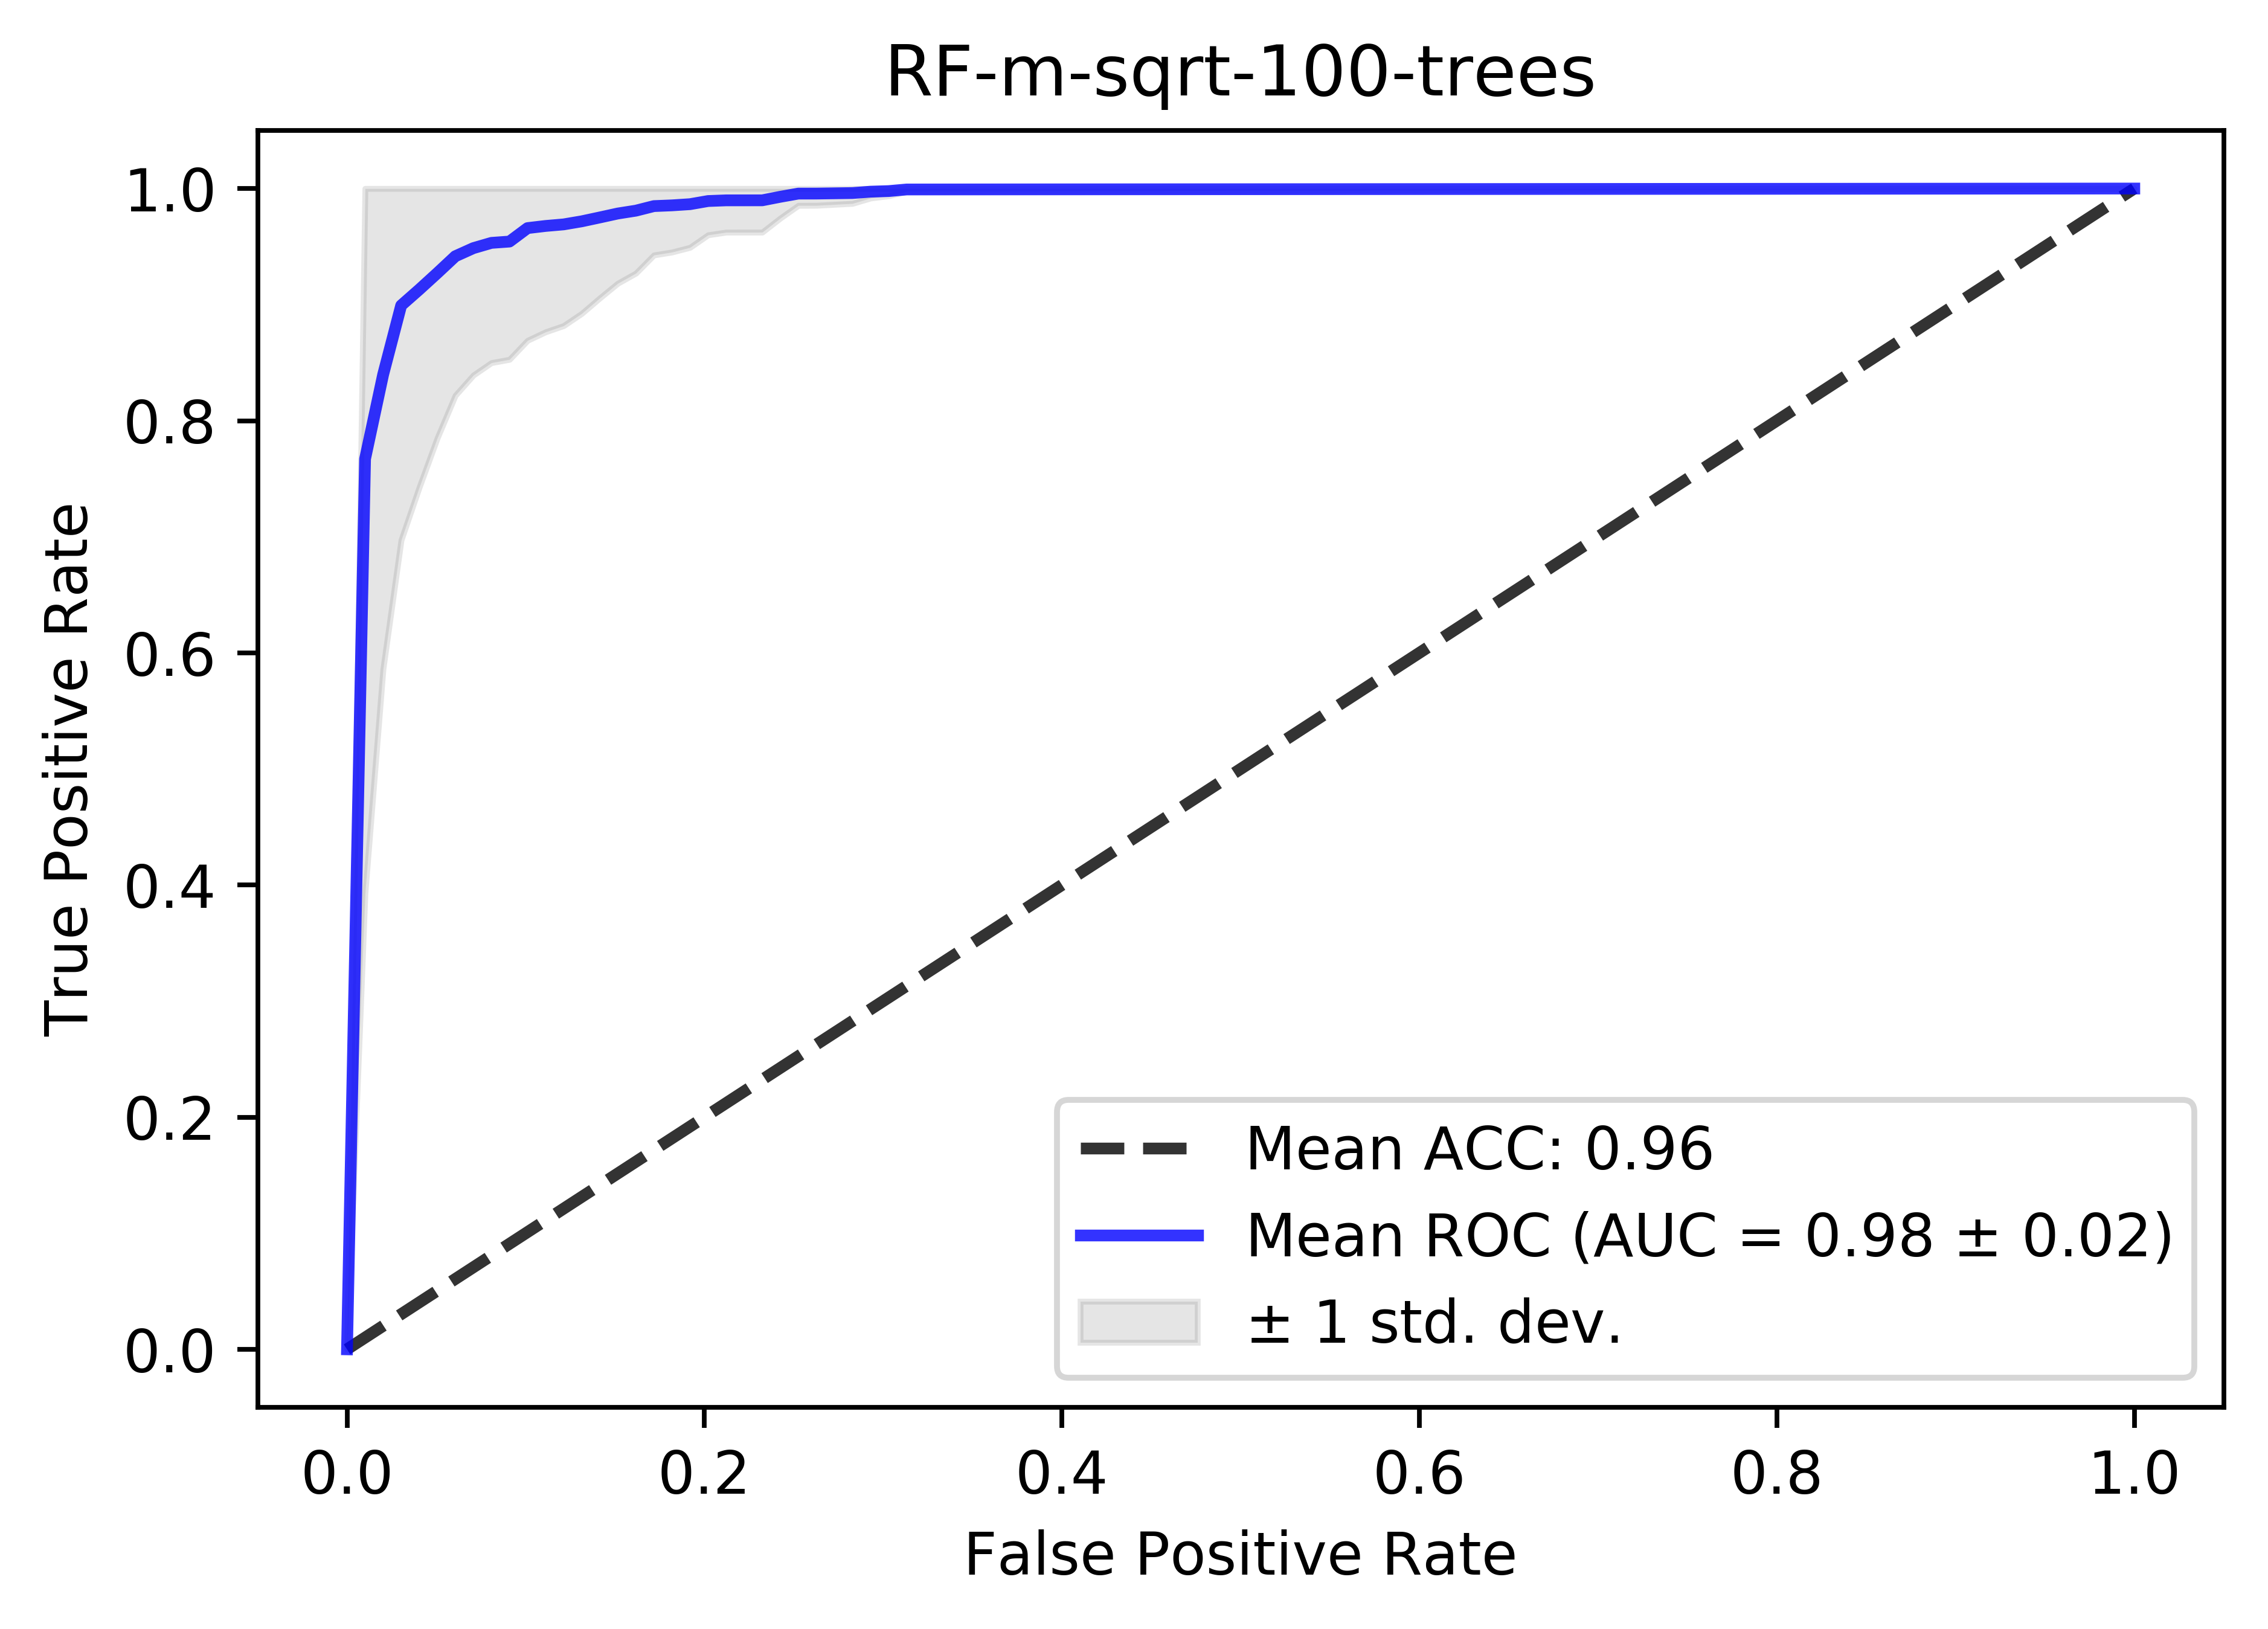
\includegraphics[width=1\textwidth]{figures/fig3}
    \end{minipage}\
    \begin{minipage}{.7\textwidth}
        \centering
        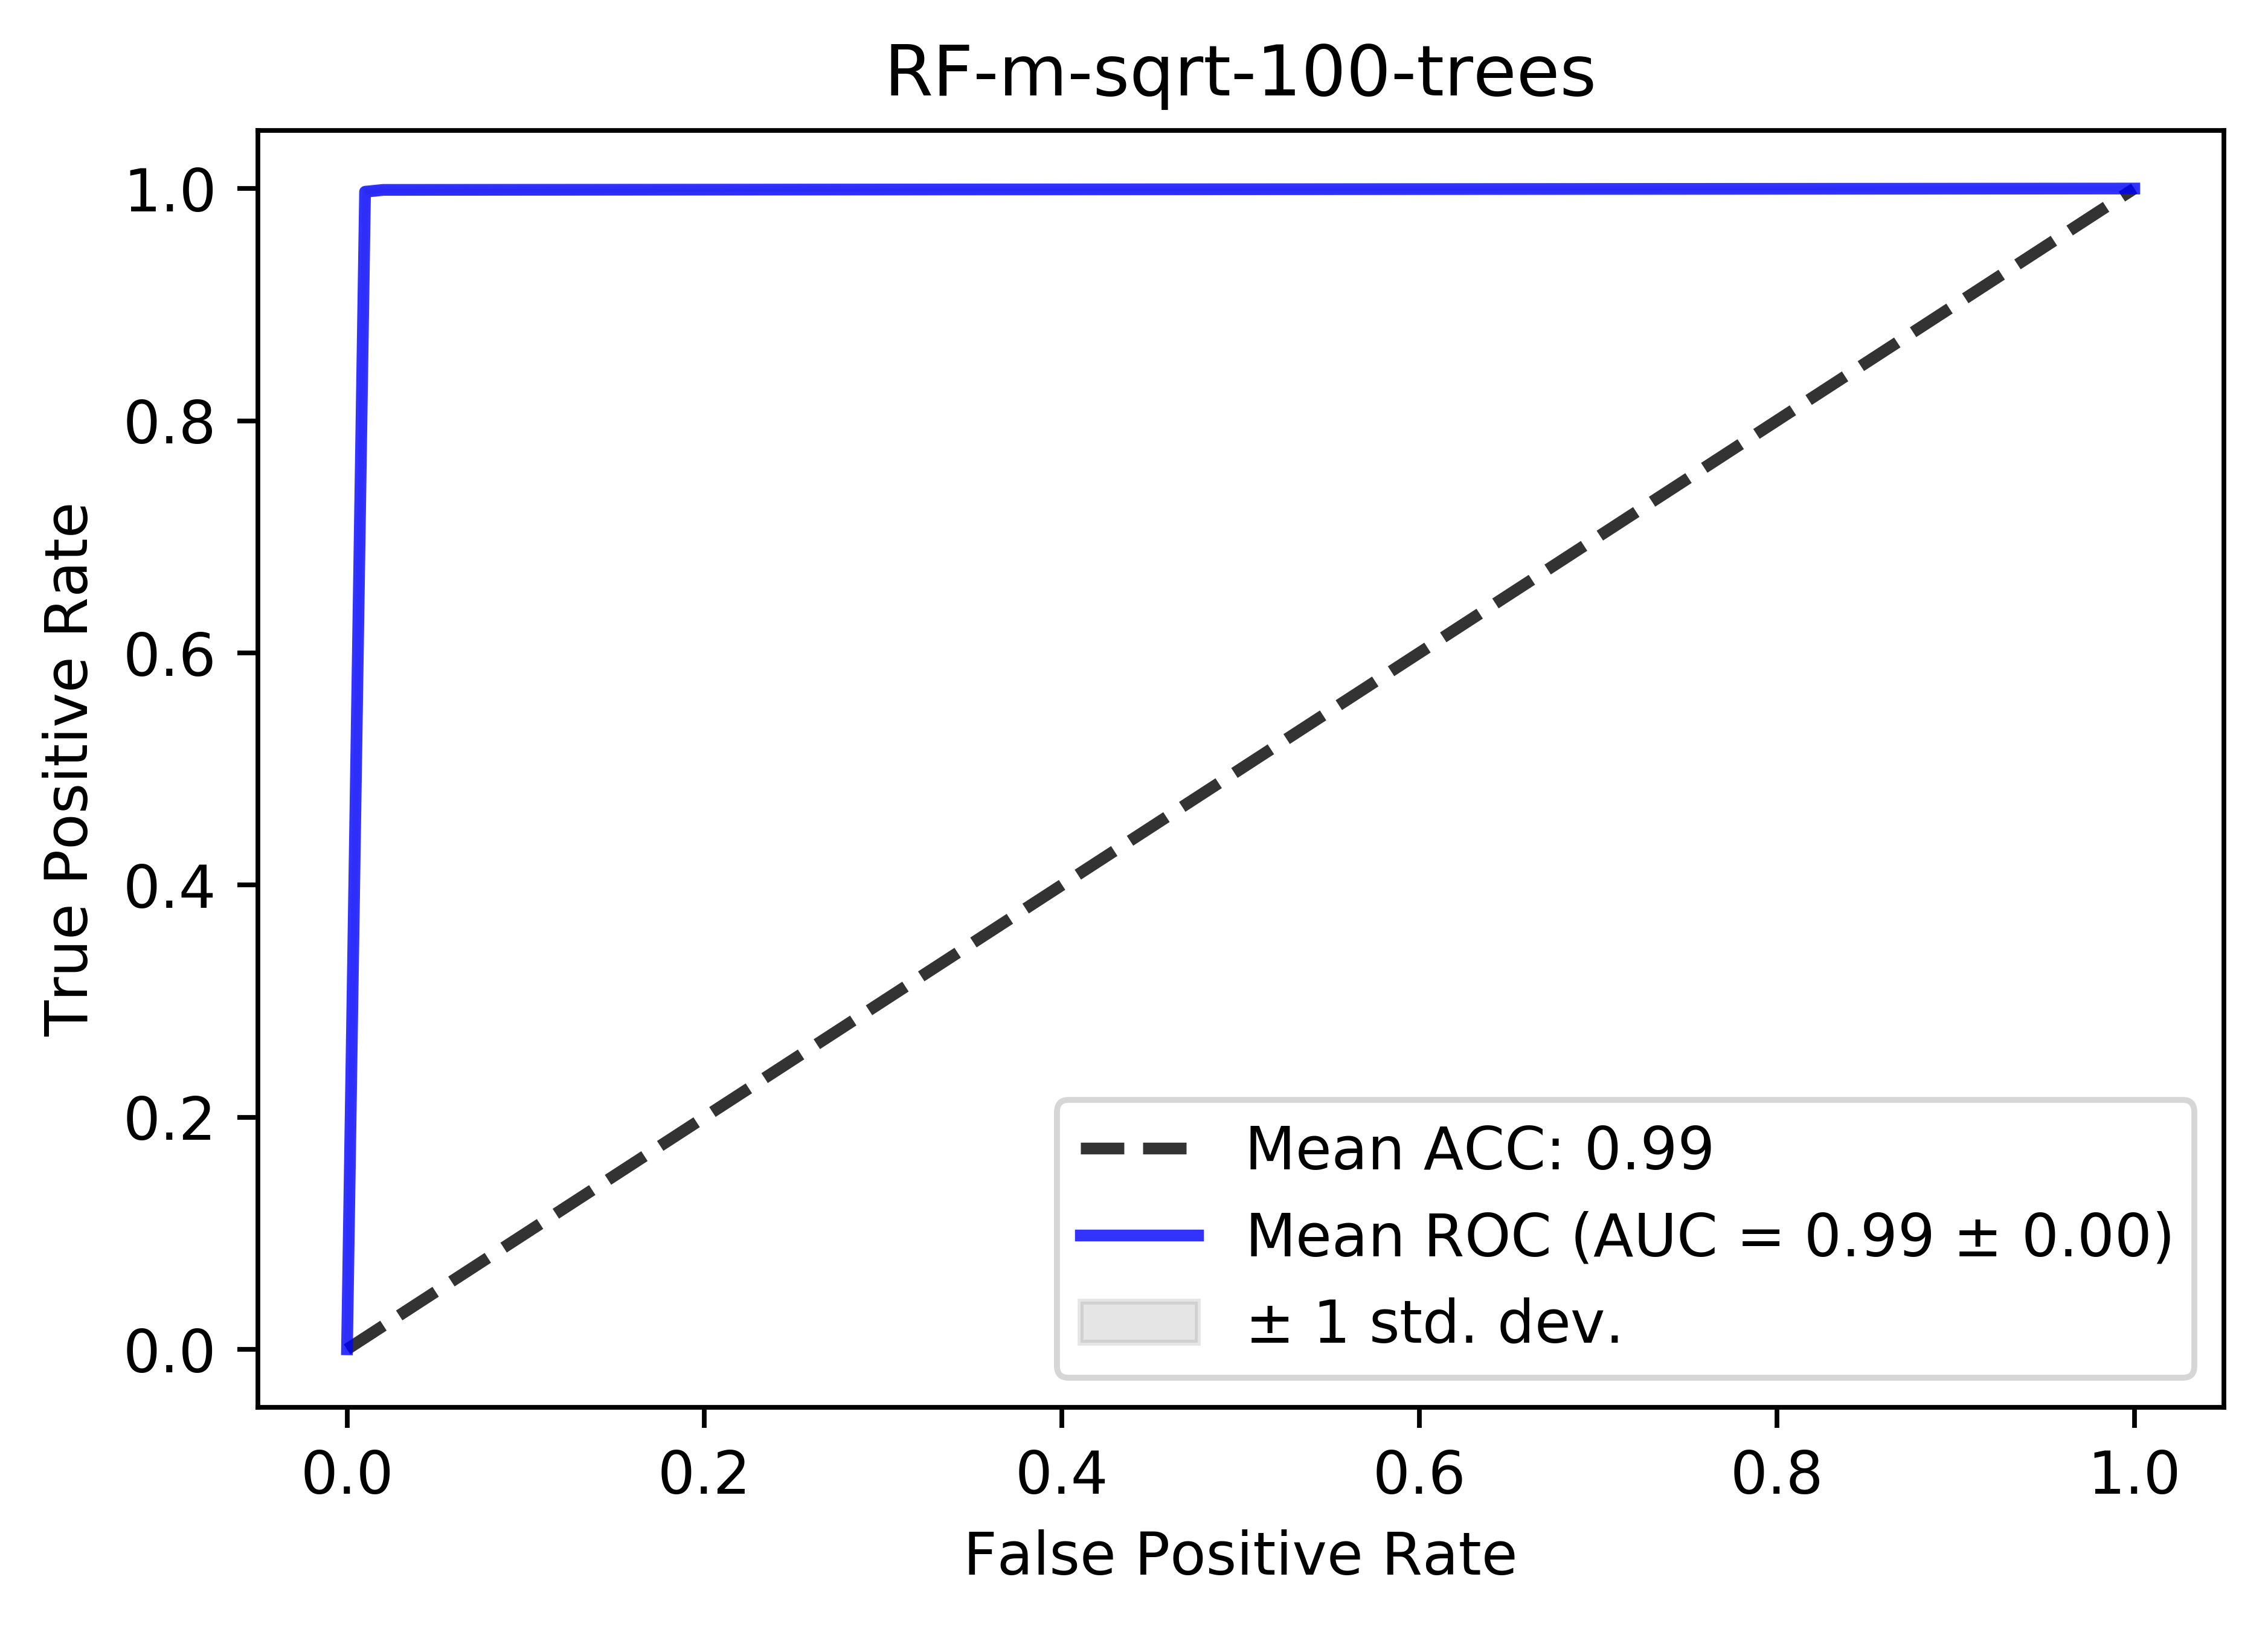
\includegraphics[width=1\textwidth]{figures/fig4}
    \end{minipage}}}
    \caption{Comparativa entre shuffling en cross validation (derecha) o dejar los datos en orden (izquierda)}
\end{figure}

Sobre estos datos se han entrenado y validado todos los modelos siguiendo el método de 10-fold cross validation tomando particiones que preserven el porcentaje de cada clase. En la \textbf{figura 3} podemos ver una comparativa entre el mismo modelo uno ajustado barajando los datos de training y el otro no, dado que nuestro conjunto de entrenamiento es una serie temporal no reordenar los datos afectaba tremendamente a las particiones causando bastante varianza entre los modelos entrenados. Por esta razón hemos barajado los datos para cada ajuste.
\\

% Hay que:

% \textcolor{blue}{Selección de las técnica (parámetrica) y valoración de la idoneidad de la misma frente a otras alternativas}

% \textcolor{blue}{Aplicación de la técnica especificando claramente que algoritmos se usan en la estimación de los parámetros, los hiperparámetros y el error de generalización.}

% \textcolor{blue}{Argumentar sobre la idoneidad de la función regularización usada (en su caso)}

\noindent \textbf{\underline{\Large Regresión Logística}}

Como método lineal hemos elegido en este caso el de regresión logística. Es un modelo que ajusta de forma bastante eficiente y rápida desde un punto de vista computacional. 
Los parámetro a ajustar para dicho modelo son la norma (penalty) y \(\lambda\), en este caso haremos uso de la inversa \(1/\lambda\). Además hemos ampliado el número máximo de iteraciones para evitar problemas de no convergencia.
Se han realizado diferentes pruebas con variantes de estos parámetros.
\begin{table}[H]
\centering
\makebox[\textwidth]{\makebox[0.8\textwidth]{%
\centering
\begin{minipage}{0.8\textwidth}
\centering
\begin{tabular}{lllll}
\textbf{Rank} & \textbf{Classifier} & \textit{Mean ACC} & \textit{Mean AUC} & \textit{STD} \\ \hline

1 & LR_{L1 - 0.01} & 0.985 & 0.993 & 0.001 \\ 
2 & LR_{L2 - 0.0001} & 0.985 & 0.992 & 0.001 \\ 
3 & LR_{L2 - 0.001} & 0.985 & 0.992 & 0.001 \\ 
4 & LR_{L2 - 0.01} & 0.985 & 0.992 & 0.001 \\ 
5 & LR_{L1 - 0.1} & 0.985 & 0.992 & 0.001 \\ 
6 & LR_{L1 - 0.0001} & 0.984 & 0.993 & 0.001 \\ 
7 & LR_{L1 - 0.001} & 0.984 & 0.993 & 0.001 \\ 
8 & LR_{L2 - 0.1} & 0.967 & 0.992 & 0.001 \\ 

\end{tabular}
\end{minipage}}}
  \footnotesize{~\\ Tabla 1. Ranking de modelos ordenados por su Accuracy, ACC (tp+tn/(P+N)), y incluyendo métricas de Area Under Curve (AUC) desviación típica del area (STD).}
\end{table}

Como podemos ver en la tabla de resultados tenemos que usando la regularización l1 que minimiza la siguiente función de coste:
\[\min_{w, c} \frac{1}{2}w^T w + C \sum_{i=1}^n \log(\exp(- y_i (X_i^T w + c)) + 1) .\]
encontramos los mejores resultados. Cabe destacar que aunque la precisión media en este caso parezca igual en todos los casos, la hemos redondeado para una mejor visualización de la tabla, pero no son iguales.

\begin{figure}[H]
\centering
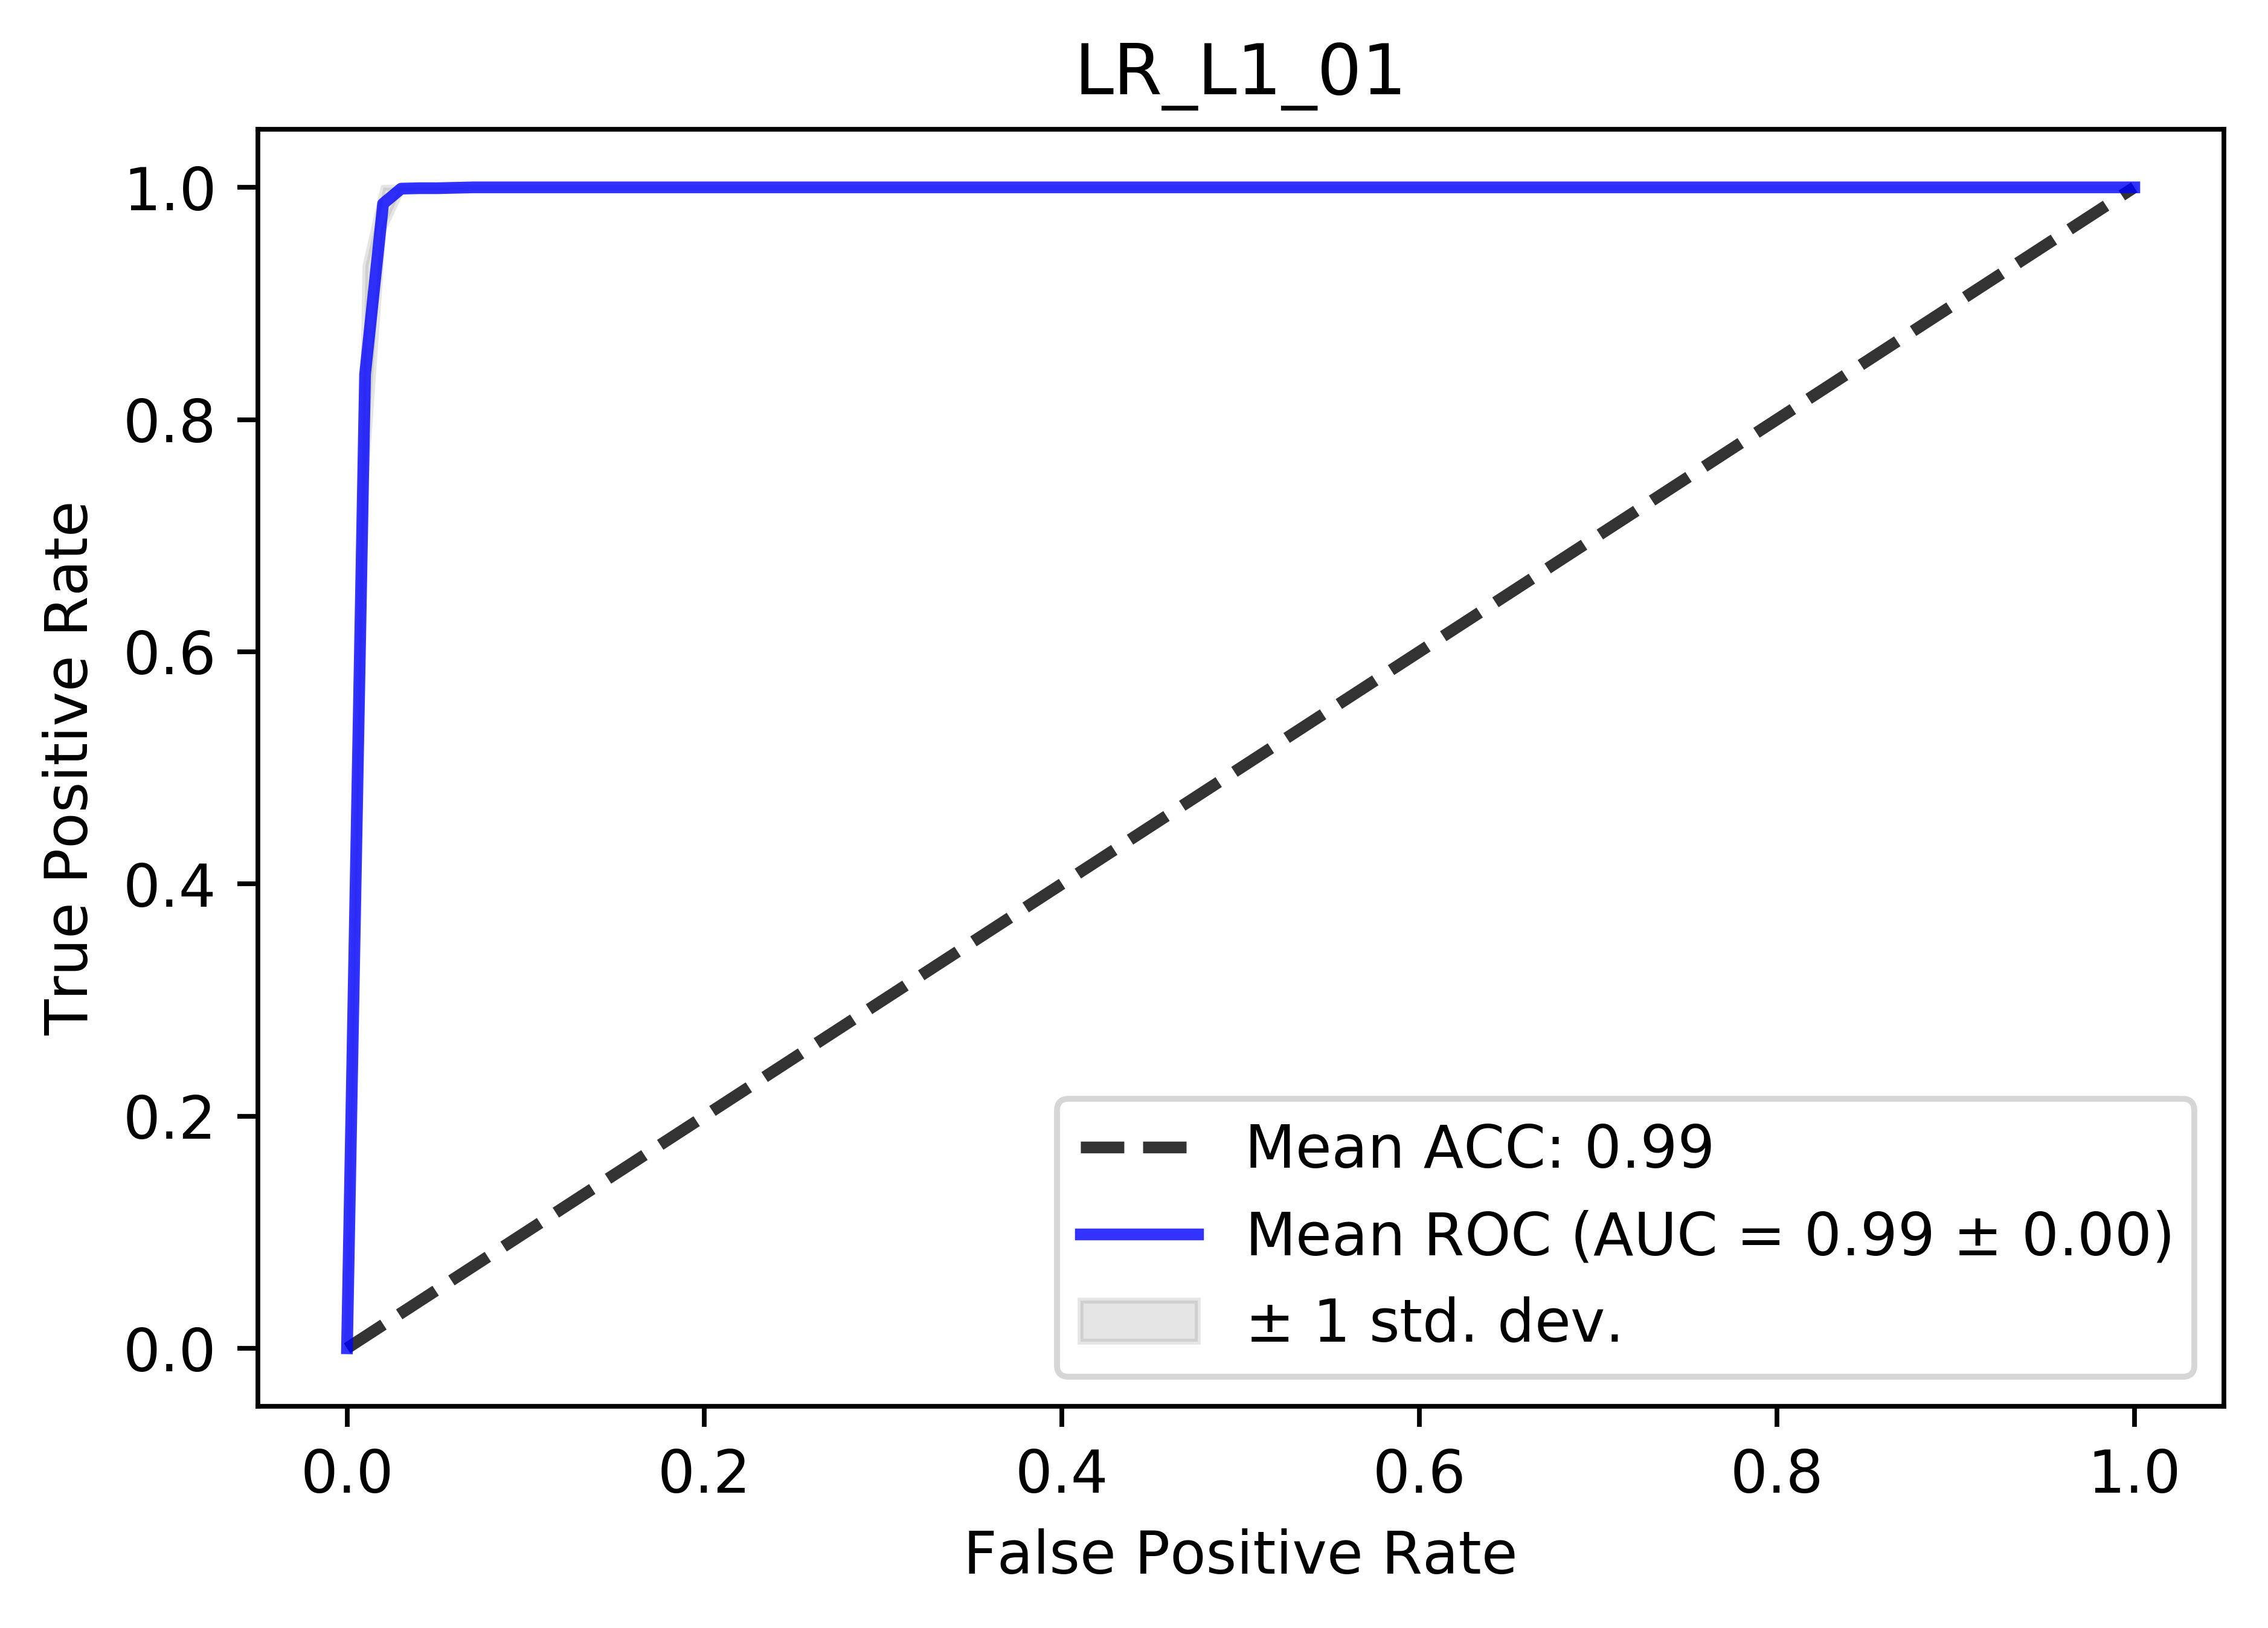
\includegraphics[width=260px]{figures/LR_L1_01_roc}
\label{fig:figure}
\caption{Mejor ajuste de Regresión Logística}
\end{figure}


~\\ ~\\
\noindent \textbf{\Large \underline{Random Forests}}

Como primer modelo no lineal probaremos a ajustar un Random Forest, este es un buen clasificador basado en el promediado de distintos arboles de clasificacion construidos sobre los datos de entrenamiento. Como hemos estudiado, es un buen modelo con poco sesgo y varianza.

Dejaremos que los arboles se puedan construir hasta el final para no introducir sesgo, dejando el parámetro \textit{max\_depth} como None.

Los parámetros a ajustar usando validación cruzada serán el número de atributos considerados para la partición \textbf{m} (\textit{max\_features}) y el número de arboles en el bosque (\textit{n\_estimators}).

\begin{table}[H]
\centering
\makebox[\textwidth]{\makebox[0.8\textwidth]{%
\centering
\begin{minipage}{0.8\textwidth}
\centering
\begin{tabular}{lllll}
\textbf{Rank} & \textbf{Classifier} & \textit{Mean ACC} & \textit{Mean AUC} & \textit{STD} \\ \hline

1 & RF-m-sqrt & 0.992 & 0.994 & 0.000 \\ 
2 & RF-m-log & 0.992 & 0.994 & 0.000 \\ 
3 & RF-m-half & 0.992 & 0.994 & 0.000 \\ 
4 & RF-m-sqrt-100-trees & 0.991 & 0.994 & 0.000 \\ 
5 & RF-m-sqrt-50-trees & 0.991 & 0.994 & 0.000 \\ 
6 & RF-m-sqrt-75-trees & 0.991 & 0.994 & 0.000 \\ 
7 & RF-m-all & 0.991 & 0.994 & 0.000 \\ 

\end{tabular}
\end{minipage}}}
  \footnotesize{~\\ Tabla 2. Resultados 10-fold CV para los modelos Random Forest.}
\end{table}

Los resultados son muy buenos en general, aunque podemos ver que los hiperparametros que habíamos decidido ajustar no afectan significativamente al ajuste del modelo. Cabe apuntar que los modelos que no indican el número de arboles tienen 25, por lo que \textbf{RF-m-sqrt-25-trees} es el modelo con el mejor ajuste.
\\

\begin{figure}[H]
\centering
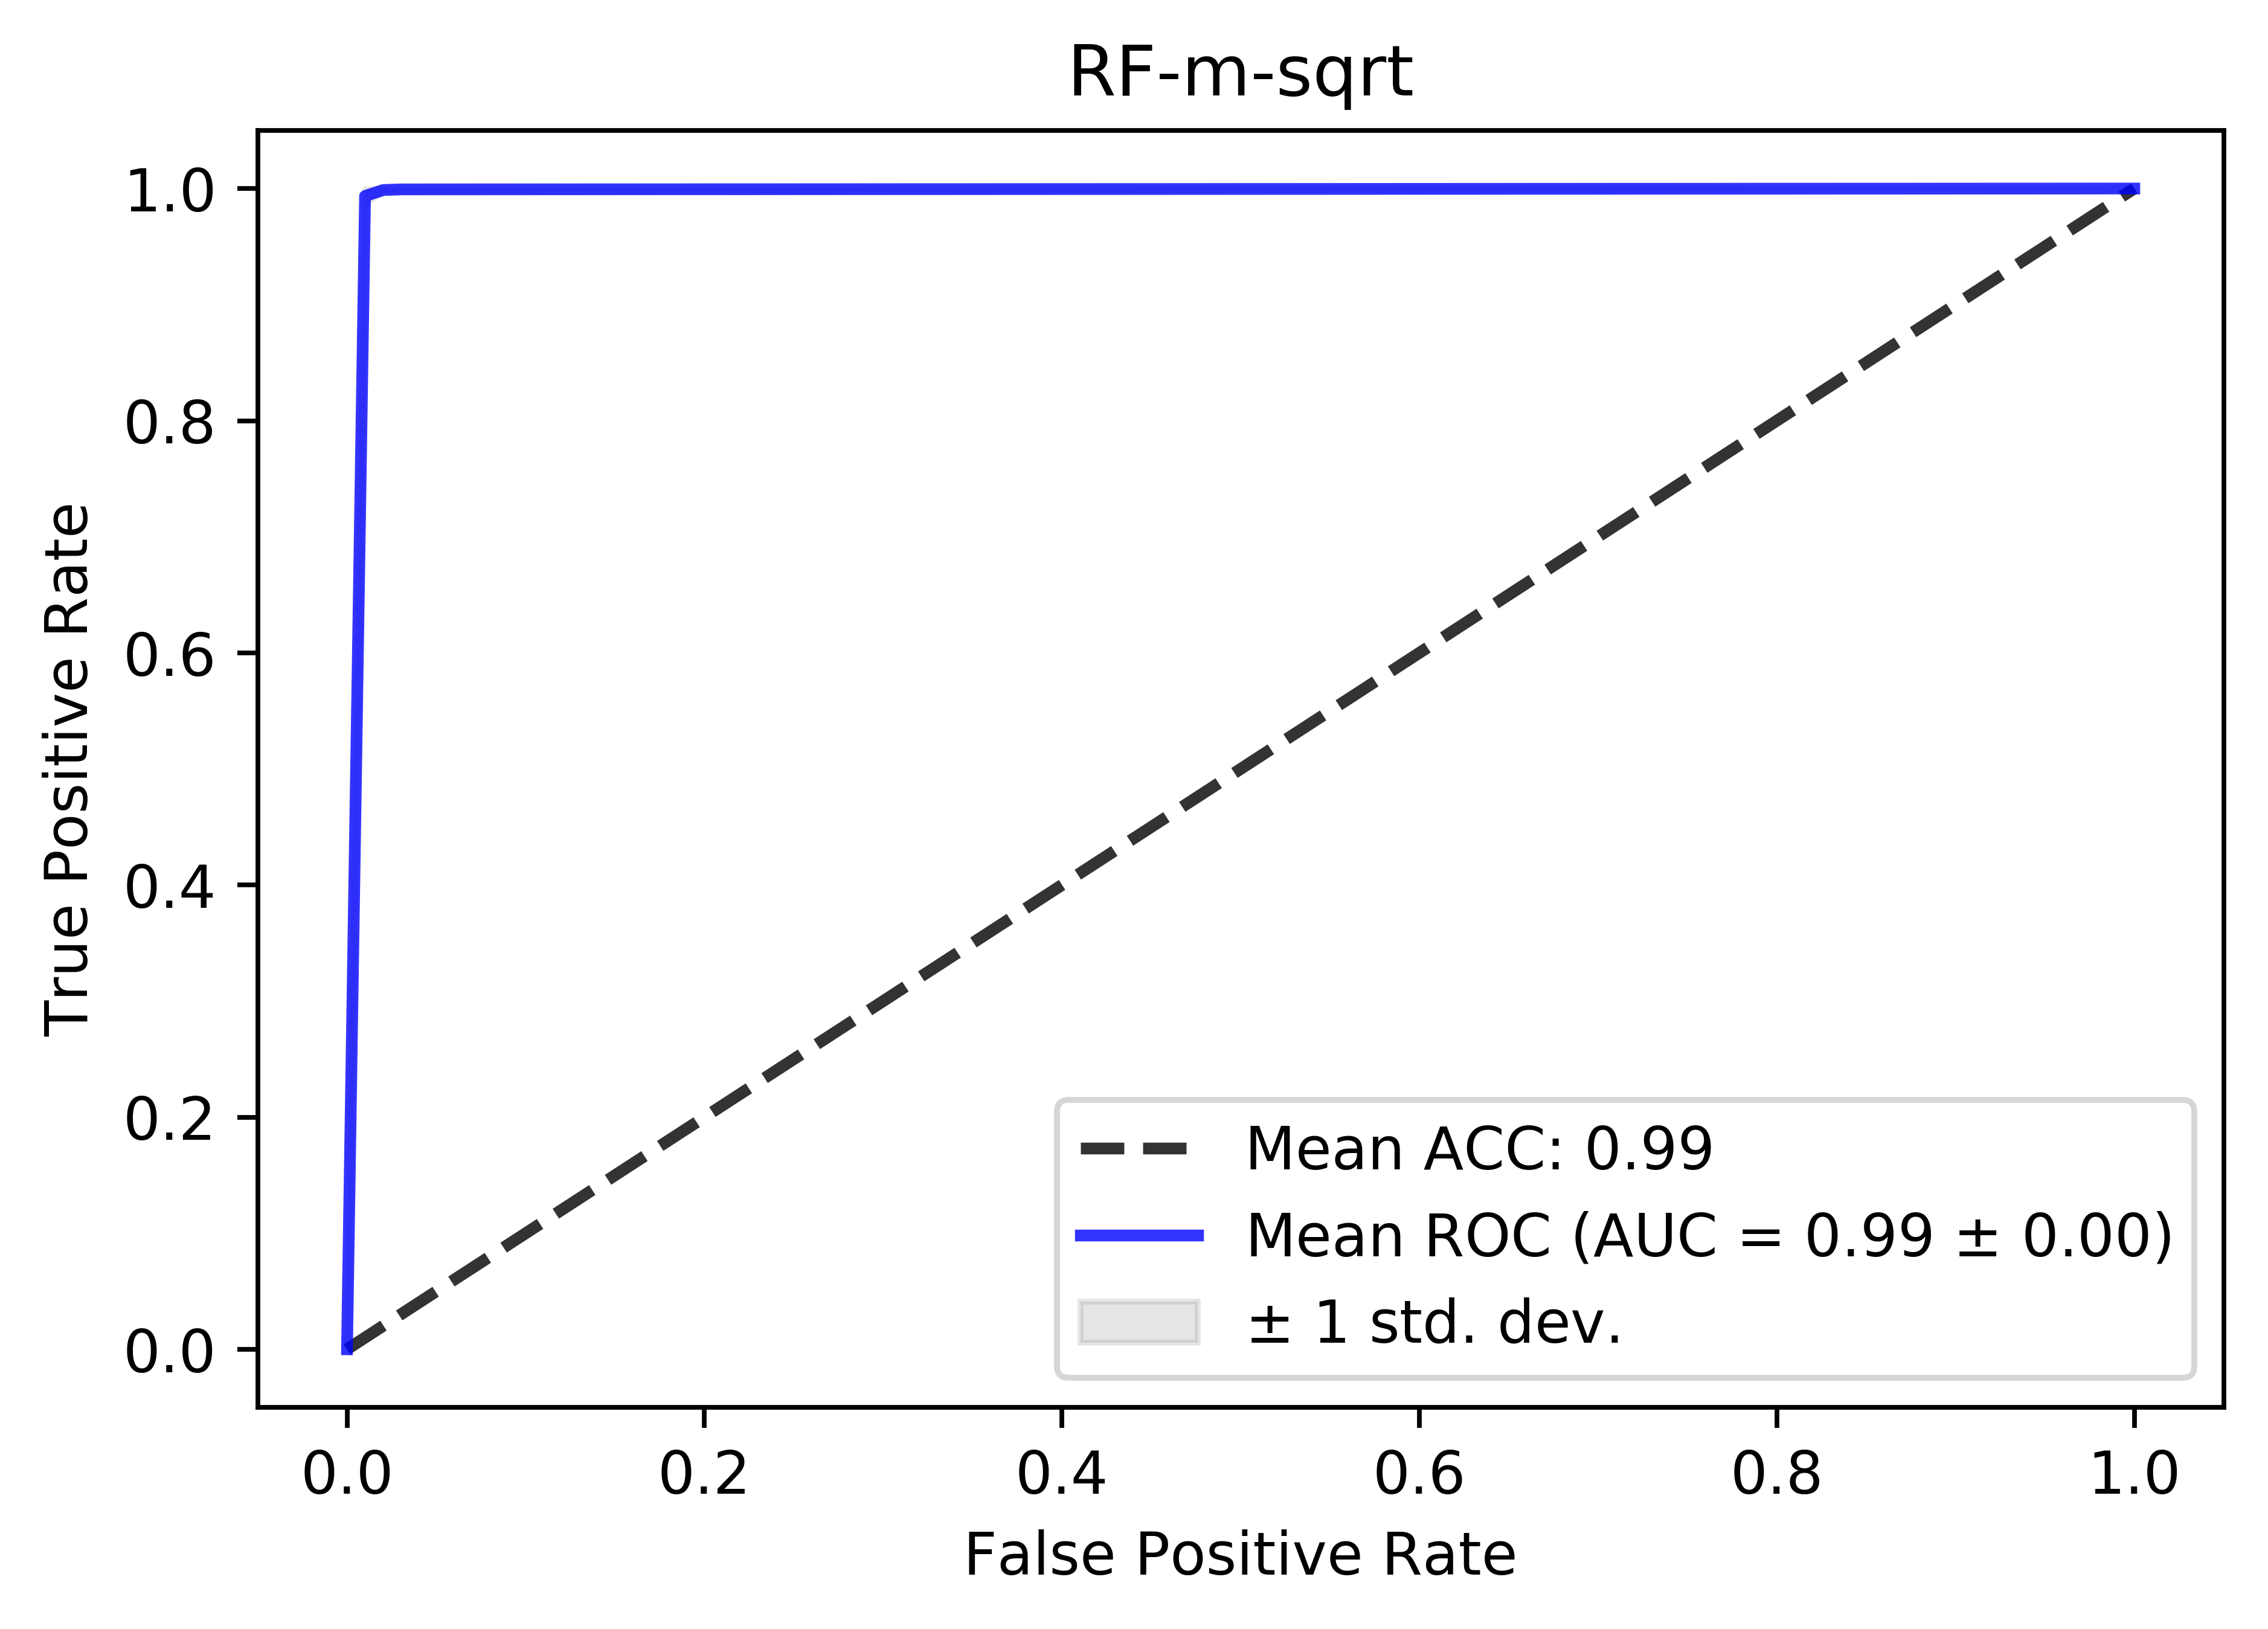
\includegraphics[width=260px]{figures/fig5}
\label{fig:figure}
\caption{Mejor ajuste de Random Forest}
\end{figure}


\noindent \textbf{\Large \underline{Redes Neuronales}}

Las redes neuronales es el modelo usado por el paper \textcolor{blue}{ref} original citado en el dataset. Los autores usaban una NN 5-6-1, con 5 nodos en la capa de entrada y una única capa oculta con 6 nodos.

Empezaremos por lo tanto considerando esta arquitectura que ya ha sido probada en este problema y ajustar el parámetro de regularización:


\begin{table}[H]
\centering
\makebox[\textwidth]{\makebox[0.8\textwidth]{%
\centering
\begin{minipage}{0.8\textwidth}
\centering
\begin{tabular}{lllll}
\textbf{Rank} & \textbf{Classifier} & \textit{Mean ACC} & \textit{Mean AUC} & \textit{STD} \\ \hline

1 & NN-5-6\_003 & 0.985 & 0.992 & 0.001 \\ 
2 & NN-5-6\_005 & 0.962 & 0.992 & 0.001 \\ 
3 & NN-5-6\_007 & 0.962 & 0.992 & 0.001 \\ 
4 & NN-5-6\_01 & 0.961 & 0.942 & 0.147 \\ 
5 & NN-5-6\_001 & 0.961 & 0.992 & 0.001 \\ 

\end{tabular}
\end{minipage}}}
  \footnotesize{~\\ Tabla 3. Resultados para la arquitectura probada con diferentes factores de regularización.}
\end{table}
\\

Comprobamos que una vez ajustado el factor de regularización $\lambda$ los resultados son excelentes con una red relativamente sencilla por lo que decidimos no aumentar la complejidad del modelo añadiendo capas ocultas o expandiendo el número de nodos de las capas actuales. 

En los resultados podemos reafirmar que NN es un modelo que tiende tremendamente al sobreajuste y por lo tanto ser gravemente penalizado al usar las particiones de validación de CV y con un poco de regularización para evitar ese sobreajuste da resultados excelentes.

\begin{figure}[H]
\centering
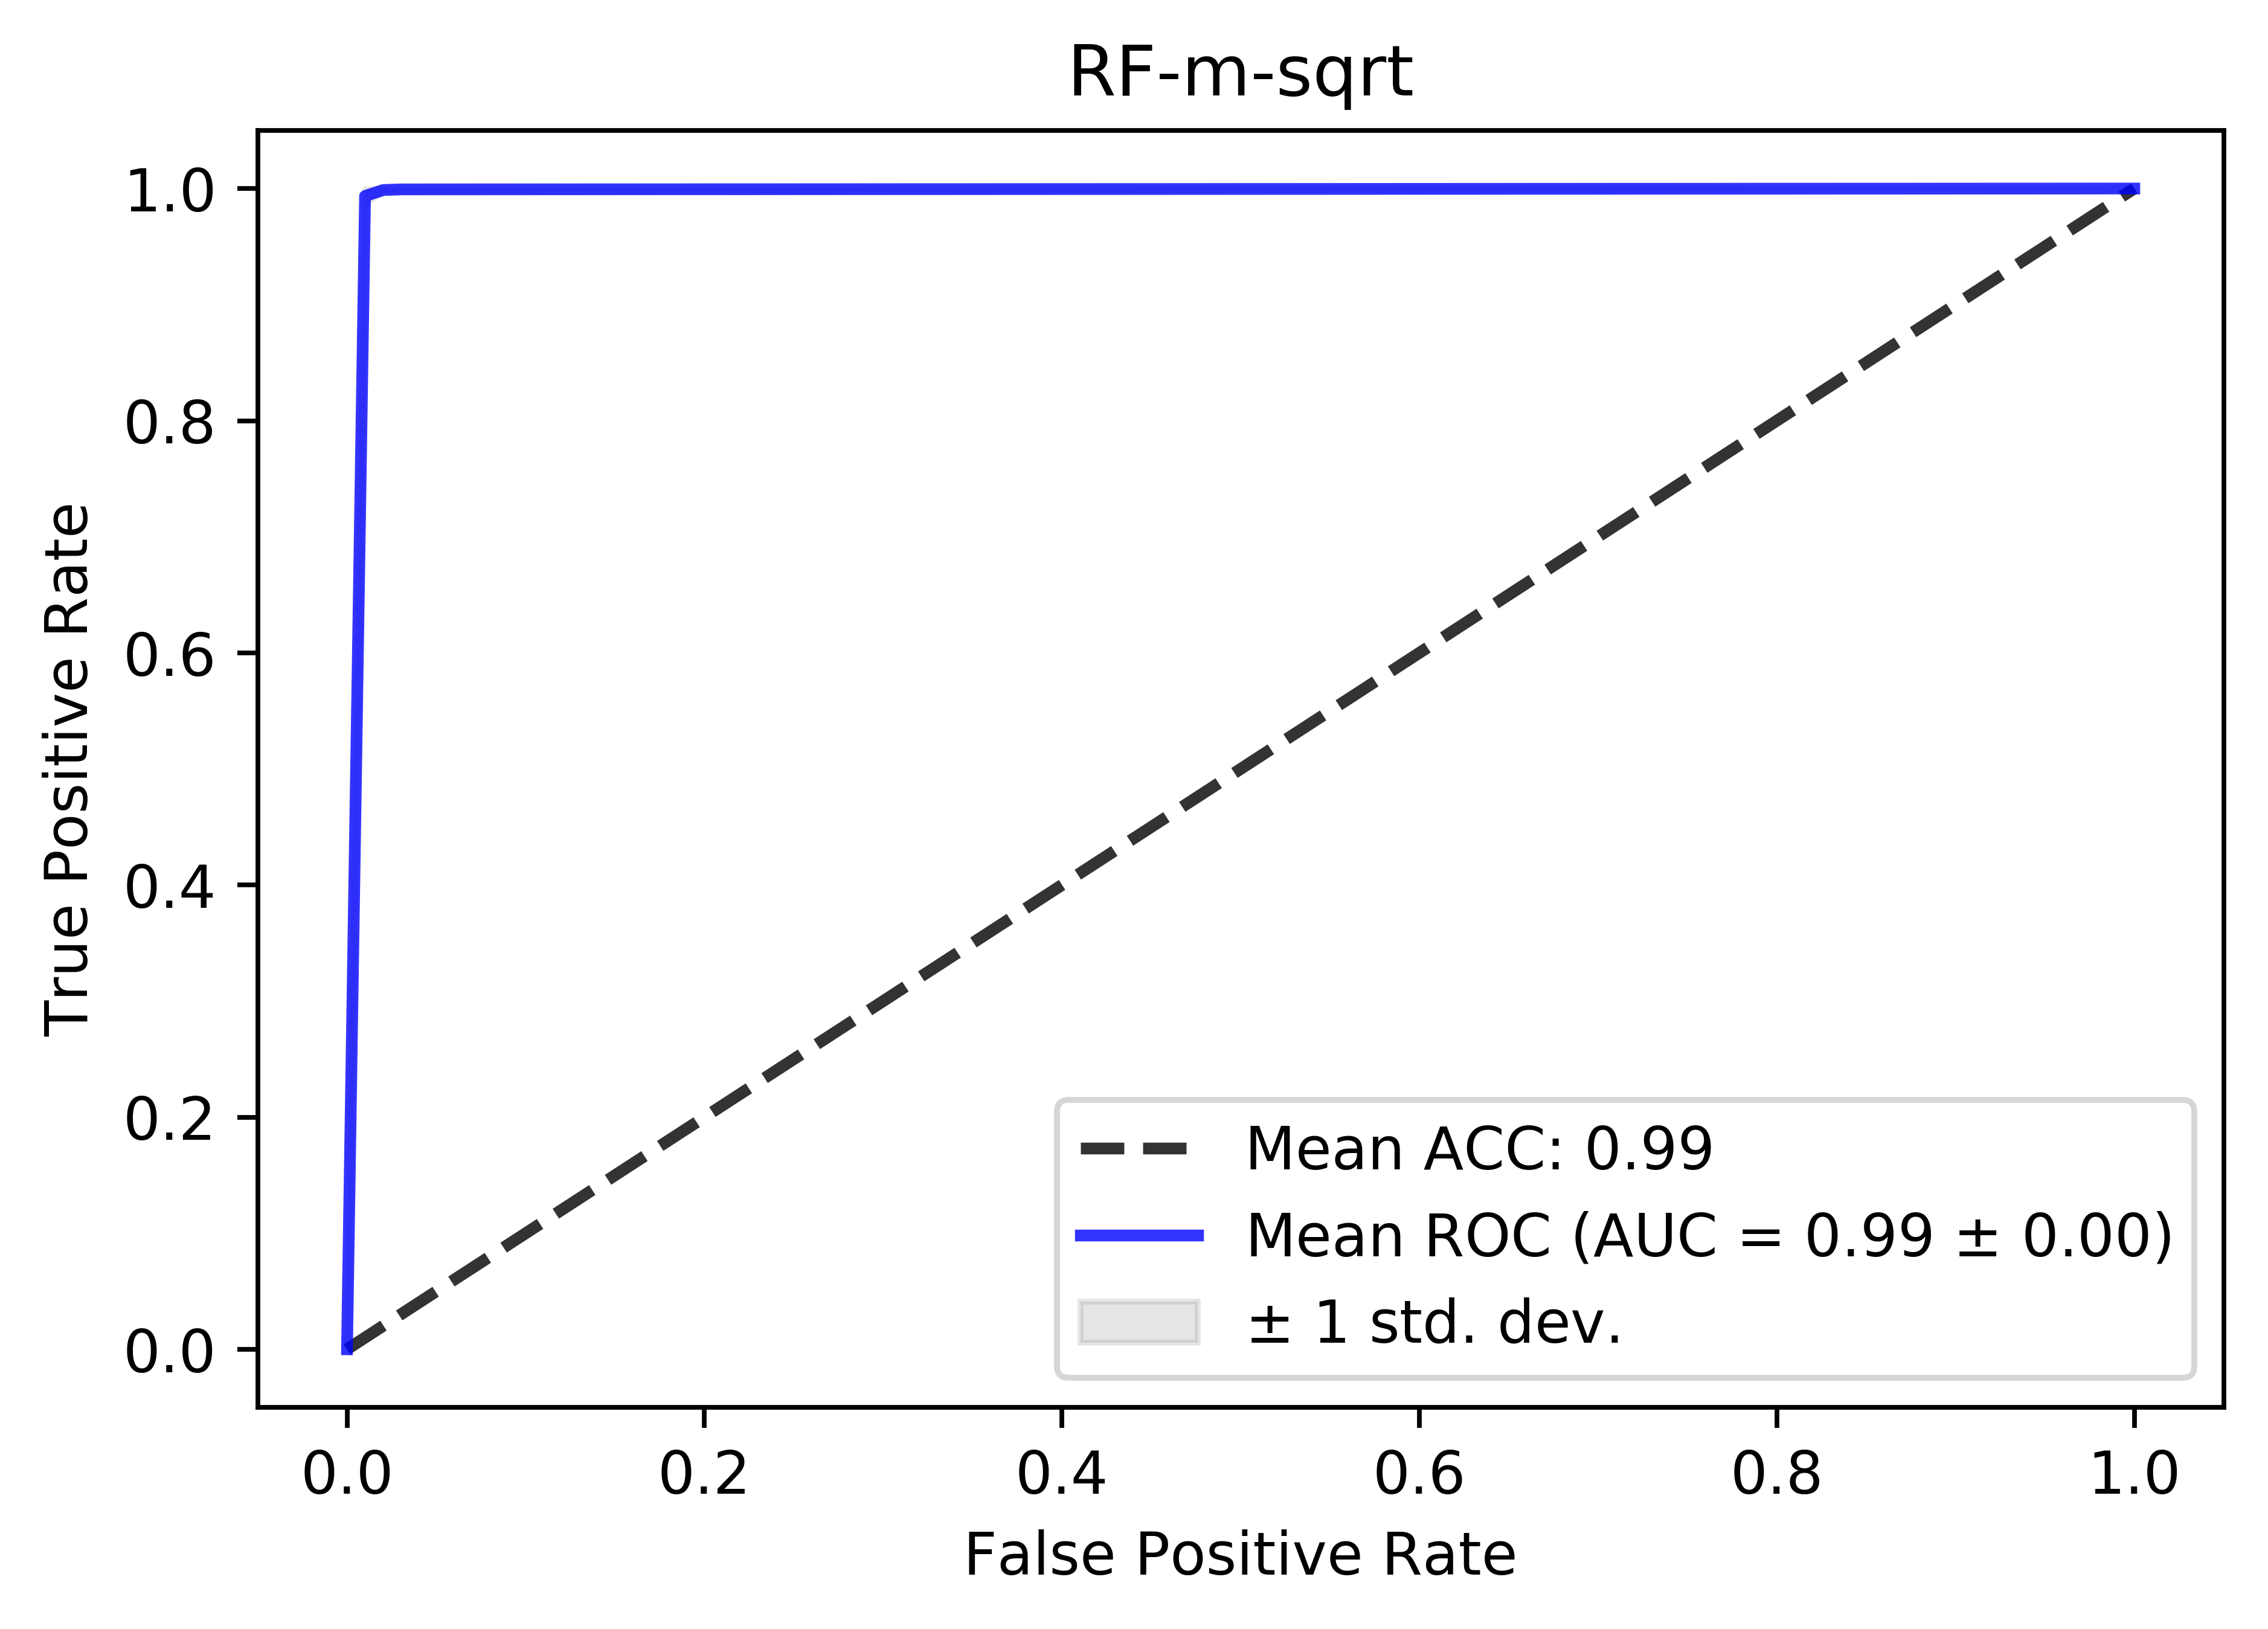
\includegraphics[width=260px]{figures/fig5}
\label{fig:figure}
\caption{Mejor ajuste con Neural Networks. Arquitectura 5-6-1 y regularización $\lambda=0.003$}
\end{figure}

\newpage

\noindent \textbf{\Large \undeline{Ada Boosting}}

Para terminar con los modelos, haremos uso de Ada Boost, una implementación de Boosting. En este tipo de técnicas se busca usar modelos débiles de los que esperamos que, al hacer uso de varias instancias de estos, se consiga un resultado global mejor que el individual de cada uno de ellos.
Para esto, AdaBoost ajusta pequeñas modificaciones de los datos que tenemos con un clasificador débil de forma iterativa. Estas modificaciones se llevan a cabo teniendo en cuenta la iteración anterior, por esto si un punto ha sido mal clasificado en la iteración anterior, en esta tendrá un peso mayor.

En este modelo tenemos que ajustar tres parámetros principalmente:
\begin{itemize}
    \item Estimador base: Se trata del clasificador débil a usar. En este caso se tratará de un árbol de decisión con profundidad 1.
    \item Número de estimadores: Es el número máximo de clasificadores débiles a usar. En este caso se ha fijado en 100, aún así si encontramos un ajuste perfecto la implementación interna de sklearn parará en ese momento.
    \item Learning rate: Este factor afectará a los pesos con los que se modifican los datos entre iteraciones.
\end{itemize}

El formato para designar cada clasificador será \(AdaBoost_{learning_rate}\):
\begin{table}[H]
\centering
\makebox[\textwidth]{\makebox[0.8\textwidth]{%
\centering
\begin{minipage}{0.8\textwidth}
\centering
\begin{tabular}{lllll}
\textbf{Rank} & \textbf{Classifier} & \textit{Mean ACC} & \textit{Mean AUC} & \textit{STD} \\ \hline

1 & AdaBoost_{1.5} & 0.987 & 0.994 & 0.000 \\ 
2 & AdaBoost_{1.8} & 0.987 & 0.994 & 0.000 \\ 
3 & AdaBoost_{1.25} & 0.987 & 0.994 & 0.000 \\ 
4 & AdaBoost_{0.5} & 0.987 & 0.994 & 0.000 \\ 
5 & AdaBoost_{1} & 0.986 & 0.994 & 0.001 \\ 
6 & AdaBoost_{0.75} & 0.986 & 0.994 & 0.001 \\ 

\end{tabular}
\end{minipage}}}
  \footnotesize{~\\ Tabla 4. Resultados para distintos parametros de AdaBoost.}
\end{table}

Aunque el número de estimadores se haya fijado a 100, nos ha parecido interesante hacer una prueba aumentando el número de estimadores a 500:
\begin{table}[H]
\centering
\makebox[\textwidth]{\makebox[0.8\textwidth]{%
\centering
\begin{minipage}{0.8\textwidth}
\centering
\begin{tabular}{lllll}
\textbf{Rank} & \textbf{Classifier} & \textit{Mean ACC} & \textit{Mean AUC} & \textit{STD} \\ \hline

1 & AdaBoost_{1.8} & 0.990 & 0.994 & 0.000 \\ 
2 & AdaBoost_{1.5} & 0.990 & 0.994 & 0.000 \\ 
3 & AdaBoost_{1} & 0.989 & 0.994 & 0.000 \\ 
4 & AdaBoost_{1.25} & 0.988 & 0.994 & 0.000 \\  
6 & AdaBoost_{0.5} & 0.988 & 0.994 & 0.000 \\  

\end{tabular}
\end{minipage}}}
  \footnotesize{~\\ Tabla 5. Resultados para distintos parametros de AdaBoost.}
\end{table}
Para las conclusiones y comparaciones, usaremos este modelo con 500 estimadores puesto supone una mejoría respecto al anterior, que será interesante comparar con el resto de modelos.

\section{Comparativa de los modelos y ajuste final}

\begin{table}[H]
\centering
\makebox[\textwidth]{\makebox[0.8\textwidth]{%
\centering
\begin{minipage}{0.8\textwidth}
\centering
\begin{tabular}{lllll}
\textbf{Rank} & \textbf{Classifier} & \textit{Mean ACC} & \textit{Mean AUC} & \textit{STD} \\ \hline
    
1 & LR\_L2\_0.01 & 0.986 & 0.990 & 0.010 \\ 
2 & AdaBoost & 0.961 & 0.985 & 0.007 \\ 
3 & MLP & 0.961 & 0.988 & 0.008 \\ 
4 & RF & 0.959 & 0.977 & 0.026 \\ 

\end{tabular}
\end{minipage}}}
  \footnotesize{~\\ Tabla 6. Comparativa de diferentes modelos ajustados.}
\end{table}

En la tabla 6 podemos ver la comparativa final entre los resultados de los diferentes modelos ajustados en un ranking en función de su accuracy.

Como modelo final por lo tanto encojemos el modelo ganador, un \textbf{Random Forest} con \textbf{25} arboles y una \textbf{m}$=\sqrt{p}$.


\section{Resultados}

Usamos una función modificada para hacer el test final que carge los datos frescos del dataset de prueba, ajuste el modelo con el training y de los resultados del ajuste:
\begin{minted}{python}
def testing(X, y, model=None, title='ROC', cv=5, plot_folds=False, \
                                args=None, normalize=True):

    X_test, y_test = read_data(filepath_test)
    
    if (normalize == True):
        X = preprocessing.normalize(X, norm='l2', axis=0)
        X_test = preprocessing.normalize(X_test, norm='l2', axis=0)
        
    np.random.seed(0)
    
    # Classification and ROC analysis
    # Run classifier with cross-validation and plot ROC curves
    cv = StratifiedKFold(n_splits=cv, shuffle=True)
    
    if model == RandomForestClassifier:
        classifier = model(n_estimators=args['rf_ntrees'], \
                           max_features=args['m'], max_depth=None)
        
    classifier.fit(X_train, y_train)
    y_pred = classifier.predict(X_test)
    acc = accuracy_score(y_test, y_pred)
    
    probas_ = classifier.predict_proba(X_test)
    # Compute ROC curve and area the curve
    fpr, tpr, thresholds = roc_curve(y_test, probas_[:, 1])
    m_auc = auc(fpr, tpr)
    std = 0.0
    
    plt.plot(fpr, tpr, lw=1, alpha=0.3, label='ROC fold %d (AUC = %0.2f)' % (i, m_auc))
    plt.xlabel('False Positive Rate')
    plt.ylabel('True Positive Rate')
    plt.title('Curva ROC del ajuste final')
    plt.show()
    return acc, m_auc, std
\end{minted}

Los resultados finales dados una vez comprobado nuestro modelo con el conjunto de test son:
\\

\noindent \textbf{Acc: 0.789} \\
\noindent \textbf{AUC: 0.5}



\bibliographystyle{alpha}
\bibliography{references}

\end{document}
